\section{Problem 1}

\subsection{a}

According to the given C code structure and the Petri Net figure, there is a risk of being in deadlock.

This situation can happen if Task A and Task B try to acquire the resources in a different order. For example, if Task B acquires resource A first and Task A acquires resource B first, a deadlock will occur because each task is waiting for the other task to release the resource it needs:

\begin{enumerate}
    \item Task A: $ p_0 $ \rightarrow(take $ r_A $) p1 \rightarrow(take $ r_B $) p2 \rightarrow p3 \rightarrow(give $ r_A $) p4 
    \subitem Task A waits $ r_A $ to continue, $ r_B $ is taken by Task A
    \item Task B: $ p_0 $ \rightarrow(take $ r_A $) p1 
    \subitem Task B waits $ r_B $ to continue, $ r_A $ is taken by Task B 
    \item Task A and B wait for each other, deadlock happens.
\end{enumerate}

\subsection{b}

\begin{figure}[H]
 \centering
 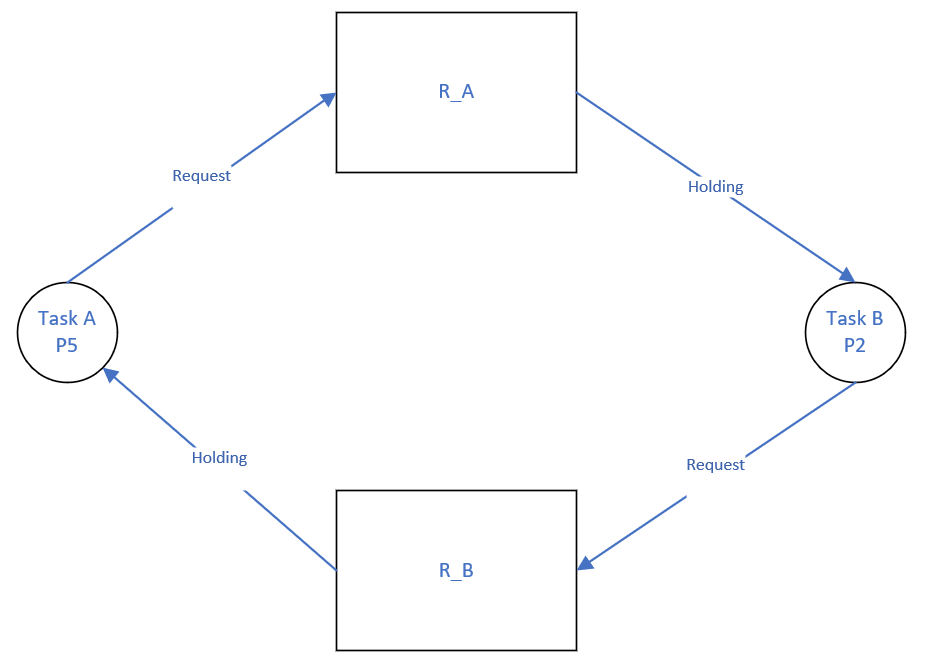
\includegraphics[width=0.7\textwidth]{images/rag.png}
 \caption{RAG graph}
 \label{rag}
\end{figure}

From figure \ref{rag}, there is a loop. And from tuturioal, if there is a cycle in the Resource Allocation Graph and each resource in the cycle provides only one instance, then the processes will be in deadlock.

(Tuturioal:https://www.geeksforgeeks.org/resource-allocation-graph-rag-in-operating-system/)

\subsection{c}

From previous analysis, the key problem is to avoid the process $ p_0 $ \rightarrow $ p_1 $ take away the $ r_A $ that process $ p_4 $ \rightarrow $ p_5 $ need, then the deadlock can be sovled.

To achieve this, using the knowledge from discreate event system, I add a new resource to the Petri Net figure, that $ p_4 $ requsts it to happen the same time $ p_1 $ requsts it to happen.

\begin{figure}[H]
 \centering
 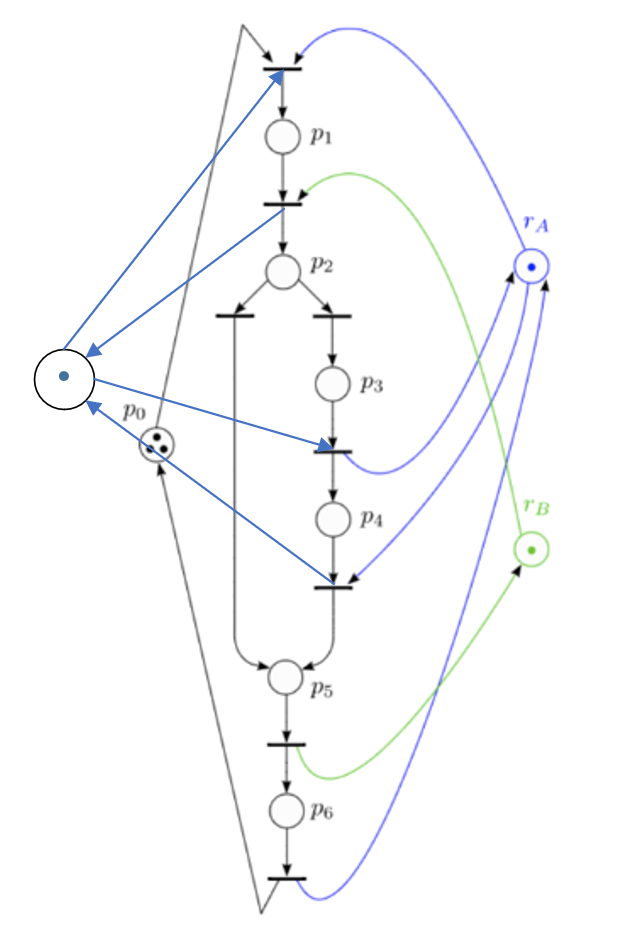
\includegraphics[width=0.7\textwidth]{images/modify.png}
 \caption{Modified Petri Net}
 \label{md}
\end{figure}

The Modified code is listed below:

\begin{lstlisting}
    #include <stdio.h>
    #include <stdlib.h>
    
    #include "FreeRTOS.h"
    #include "task.h"
    #include "semphr.h"
    
    xTaskHandle task_a_handle;
    xTaskHandle task_b_handle;
    xTaskHandle task_c_handle;
    
    SemaphoreHandle_t resource_a;
    SemaphoreHandle_t resource_b;
    SemaphoreHandle_t resource_c;
    
    void the_task(void *pvParameters)
    {
        while (1)
        {
            xSemaphoreTake(resource_c, portMAX_DELAY);//Take resouce c to go into p1
            xSemaphoreTake(resource_a, portMAX_DELAY);
            ...
            xSemaphoreTake(resource_b, portMAX_DELAY);
            xSemaphoreGive(resource_c, portMAX_DELAY);//Only protect p1, after p1 give it out
            ...
            if (...)
            {
                ...
                xSemaphoreTake(resource_c, portMAX_DELAY);//Take resouce c to go into p4
                xSemaphoreGive(resource_a);
                ...
                xSemaphoreTake(resource_a, portMAX_DELAY);
                xSemaphoreGive(resource_c, portMAX_DELAY);//After p4 give it out
                ...
            }
            xSemaphoreGive(resource_b);
            ...
            xSemaphoreGive(resource_a);
            ...
        }
    }
    
    int main(int argc, char **argv)
    {
        resource_a = xSemaphoreCreateMutex();
        resource_b = xSemaphoreCreateMutex();
        resource_c = xSemaphoreCreateMutex();
        xTaskCreate(the_task, "Task 1", configMINIMAL_STACK_SIZE, NULL, 1, &task_a_handle);
        xTaskCreate(the_task, "Task 2", configMINIMAL_STACK_SIZE, NULL, 1, &task_b_handle);
        xTaskCreate(the_task, "Task 3", configMINIMAL_STACK_SIZE, NULL, 1, &task_c_handle);
        
    
        vTaskStartScheduler();
        for( ;; );
    }
    
    
\end{lstlisting}

